[102 r\textsuperscript{o}]  in aqua sparsae collidantur, aut inter concussionem  rimas communicationis inveniant ad se colligendum  potest etiam ictus tubo impactus ex ipsis ejus  lateribus excutere aeris nonnihil unde bulla generetur.  Cur \textso{Experim. 3.} spiritus vini\protect\index{Sachverzeichnis}{spiritus!vini} \edtext{promtius  bullis}{\lemma{vini}\Afootnote{ \textit{ (1) }\ plus bullarum \textit{ (2) }\ promtius  bullis \textit{ L}\protect\rule[0cm]{5cm}{0cm}}} purgetur, alia quaestio est, caeterae Experim. 3.  circumstantiae ex dictis patent.\edtext{}{\lemma{patent.}\Bfootnote{\textsc{Chr. Huygens, }\cite{00062}a.a.O., S.~136f. (\textit{HO} VII, S.~203f.).}} Cur Experim. 4.  bulla resorbeatur, ubi primum ratio ejus exprimendae  cessavit per se patet.\edtext{}{\lemma{patet.}\Bfootnote{\textsc{Chr. Huygens, }\cite{00062}a.a.O., S.~137\textendash139 (\textit{HO} VII, S.~204f.).}} De Experimento 5. et 6.  duarum Tabularum politarum\protect\index{Sachverzeichnis}{tabulae!politae}, Siphonis\protect\index{Sachverzeichnis}{sipho} item  iniquicruri, jam dictum est, cur necessario in  Recipiente exhausto non minus evenerit.\edtext{}{\lemma{evenerit.}\Bfootnote{\textsc{Chr. Huygens, }\cite{00062}a.a.O., S.~139f. (\textit{HO} VII, S.~205f.).%\protect\rule[0mm]{10cm}{0mm}
}}
\pend  
%Zeitzauskommentiert\clearpage
%\begin{center}                    
%                \protect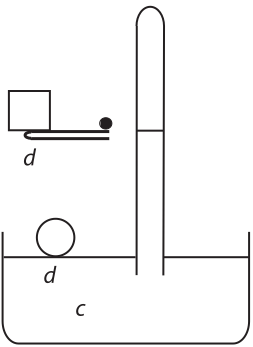
\includegraphics[width=0.31\textwidth]{images/37_3_102r1}
%                \protect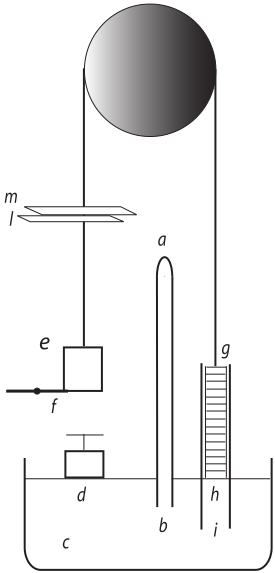
\includegraphics[width=0.4\textwidth]{images/37_3_102r2}\\\textit{[Fig. 2, gestr.]}\hspace{3cm}\textit{[Fig. 3]}\rule[0cm]{1cm}{0cm}
%                        %\caption{Bildbeschreibung}
%                        \end{center}
%                        \clearpage
%                        %@ @ @ Dies ist eine Abstandszeile - fuer den Fall, dass mehrere figures hintereinander kommen, ohne dass dazwischen laengerer Text steht. Dies kann zu einer Fahlermeldung fuehren. @ @ @ \\
                  \pstart Nunc alia Experimenta proponam, \edtext{nova}{\lemma{proponam,}\Afootnote{ \textit{ (1) }\ quae sententiam  meam plane \textit{ (2) }\ quorum eventum \textit{ (3) }\ nova \textit{ L}}} nec hactenus  sumta, lucem\protect\index{Sachverzeichnis}{lux} tamen huic argumento insignem  ut spero allatura. Et primum modum generalem  proponam cujus ope Motus varii in Recipiente 
 Magdeburgico\protect\index{Sachverzeichnis}{Recipiens!Magdeburgicum} procurari possunt, ita ut eum  concuti, aut aperiri \edtext{necesse}{\lemma{aperiri}\Afootnote{ \textit{ (1) }\ , aut magnetem\protect\index{Sachverzeichnis}{magnes|textit} \textit{ (2) }\ necesse \textit{ L}}} non sit.\footnote{\textit{In der rechten Spalte}: \textso{Experim. 5.}} Cum aqua \edtext{liquorve alius}{\lemma{}\Afootnote{liquorve alius \textit{ erg.~L}}} ex Tubo \edtext{\textit{ab}}{\lemma{\textit{ab}}\Afootnote{ \textit{ erg.} \textit{ L}}} in vas subjectum \edtext{\textit{c}}{\lemma{}\Afootnote{\textit{c} \textit{ erg.} \textit{ L}}} descendat  proportione aeris, hinc fit ut vas  subjectum magis magisque impleatur, ac per consequens  corpus in eo natans assurgat. Potest \edtext{autem  surgendo}{\lemma{autem}\Afootnote{ \textit{ (1) }\ illidendo \textit{ (2) }\   surgendo \textit{ L}}} alia corpora movere, aut suspensa Elateria\protect\index{Sachverzeichnis}{elaterium}  ponderave attactu liberare ad effectus varios a nobis designatos  producendos. Hoc jam ad effectum antliae\protect\index{Sachverzeichnis}{antlia} in Recipiente  exhausto praestandum ita applicetur.\footnote{\textit{In der rechten Spalte}: \textso{Experim. 6.}} Esto pondus \textit{e} 
 levi  corporis \textit{d} assurgentis attactu a fulcimento \textit{f} liberandum  hoc labendo embolum\protect\index{Sachverzeichnis}{embolus} \textit{gh} antliae\protect\index{Sachverzeichnis}{antlia} \textit{gi} extrahet, aquamque \edtext{aere scilicet purgatam}{\lemma{aere}\Afootnote{ scilicet purgatam \textit{ erg.} \textit{ L}}}  ex [\textit{gi}]\edtext{}{\Afootnote{\textit{hi}\textit{\ L \"{a}ndert Hrsg. } }} in \textit{gh} attollet. Quod si fiet, ut ego quidem  futurum esse praedicere ausim, jam non erit dubitandum, ab aeris pressione\protect\index{Sachverzeichnis}{pressio!aeris} quae in Baroscopio\protect\index{Sachverzeichnis}{baroscopium} sentitur antliae\protect\index{Sachverzeichnis}{antlia} effectum non pendere, \edtext{quod}{\lemma{}\Afootnote{quod  \textbar\ hactenus \textit{ gestr.}~\textbar\ tamen \textit{ L}}} tamen  non Pascalio\protect\index{Namensregister}{\textso{Pascal} (Pascalius), Blaise 1623\textendash 1662} tantum, sed et multis aliis nostri temporis  philosophis indubitatum videbatur. Cum enim \edtext{aquam per antliam elevabilem,}{\lemma{enim}\Afootnote{ \textit{ (1) }\ calculum  aquae per antliam\protect\index{Sachverzeichnis}{antlia|textit} attollendae, cum \textit{ (2) }\ aquam per antliam elevabilem, \textit{ L}}}  ejusdem circiter ponderis esse \edtext{cernerent}{\lemma{}\Afootnote{cernerent \textit{ erg.} \textit{ L}}} cum Mercurio\protect\index{Sachverzeichnis}{mercurius}  in Baroscopio\protect\index{Sachverzeichnis}{baroscopium} suspenso;\edtext{}{\lemma{}\Afootnote{suspenso;  \textbar\ assumta scilicet aequali  Tuborum \textit{ gestr.}\ \textbar\ seu \textit{ L}}} seu quod idem est eam esse \edtext{circiter}{\lemma{}\Afootnote{circiter \textit{ erg.} \textit{ L}}} rationem altitudinis \edtext{aquae in antlia\protect\index{Sachverzeichnis}{antlia}}{\lemma{}\Afootnote{aquae in antlia\protect\index{Sachverzeichnis}{antlia} \textit{ erg.} \textit{ L}}}  (32 pedum) ad altitudinem Mercurii\protect\index{Sachverzeichnis}{mercurius} (27 pollicum) in Baroscopio\protect\index{Sachverzeichnis}{baroscopium} quae est gravitatis\protect\index{Sachverzeichnis}{gravitas} Mercurii\protect\index{Sachverzeichnis}{mercurius} specificae  ad gravitatem\protect\index{Sachverzeichnis}{gravitas} aquae specificam id est circiter ut 14. ad 1.  Jam non dubitabant, ut Baroscopii\protect\index{Sachverzeichnis}{baroscopium}, ita et antliae\protect\index{Sachverzeichnis}{antlia} effectus  in aere exhausto vacuove cessaturos, in qua tamen re  eos opinio fefellit. Nam cum Sipho\protect\index{Sachverzeichnis}{sipho} iniquicrurus (in quo  aqua cruris majoris emboli\protect\index{Sachverzeichnis}{embolus} \edtext{liquidi proprio pondere}{\lemma{liquidi}\Afootnote{ proprio pondere \textit{ erg.} \textit{ L}}} extracti loco haberi  potest ad aquam cruris majoris elevandam) effectum  suum in vacuo praestet,\edtext{}{\lemma{}\Afootnote{praestet,  \textbar\ idem \textit{ gestr.}\ \textbar\ de \textit{ L}}} de antlia\protect\index{Sachverzeichnis}{antlia} \edtext{seu embolo\protect\index{Sachverzeichnis}{embolus} solido}{\lemma{}\Afootnote{seu embolo\protect\index{Sachverzeichnis}{embolus} solido \textit{ erg.} \textit{ L}}} non erit dubitandum.  Eodem modo fiat \textso{Experimentum,} an tanto pondere opus  sit ad duas laminas divellendas \edtext{in vacuo}{\lemma{}\Afootnote{in vacuo \textit{ erg.} \textit{ L}}} quanto opus est in pleno.\footnote{\textit{In der rechten Spalte}: \textso{Experim. 7.}} Suspendatur scilicet pondus \textit{e} dum attactu corporis \textit{d}  liberatum laminas \textit{l} \textit{m} divellat. Arbitror \edtext{in summa}{\lemma{}\Afootnote{in summa \textit{ erg.} \textit{ L}}} discrimen  ad rem pertinens fore nullum, et quod futurum est ab alia fore  causa, ut quod pondus omne in vacuo plus ponderat quam in pleno, \edtext{similibusque.}{\lemma{similibusque.}\Afootnote{ \textit{ (1) }\ Sed ut \textit{ (2) }\ Mirabitur \textit{ L}}}